%% template.tex
%% from
%% bare_conf.tex
%% V1.4b
%% 2015/08/26
%% by Michael Shell
%% See:
%% http://www.michaelshell.org/
%% for current contact information.
%%
%% This is a skeleton file demonstrating the use of IEEEtran.cls
%% (requires IEEEtran.cls version 1.8b or later) with an IEEE
%% conference paper.
%%
%% Support sites:
%% http://www.michaelshell.org/tex/ieeetran/
%% http://www.ctan.org/pkg/ieeetran
%% and
%% http://www.ieee.org/

%%*************************************************************************
%% Legal Notice:
%% This code is offered as-is without any warranty either expressed or
%% implied; without even the implied warranty of MERCHANTABILITY or
%% FITNESS FOR A PARTICULAR PURPOSE!
%% User assumes all risk.
%% In no event shall the IEEE or any contributor to this code be liable for
%% any damages or losses, including, but not limited to, incidental,
%% consequential, or any other damages, resulting from the use or misuse
%% of any information contained here.
%%
%% All comments are the opinions of their respective authors and are not
%% necessarily endorsed by the IEEE.
%%
%% This work is distributed under the LaTeX Project Public License (LPPL)
%% ( http://www.latex-project.org/ ) version 1.3, and may be freely used,
%% distributed and modified. A copy of the LPPL, version 1.3, is included
%% in the base LaTeX documentation of all distributions of LaTeX released
%% 2003/12/01 or later.
%% Retain all contribution notices and credits.
%% ** Modified files should be clearly indicated as such, including  **
%% ** renaming them and changing author support contact information. **
%%*************************************************************************


% *** Authors should verify (and, if needed, correct) their LaTeX system  ***
% *** with the testflow diagnostic prior to trusting their LaTeX platform ***
% *** with production work. The IEEE's font choices and paper sizes can   ***
% *** trigger bugs that do not appear when using other class files.       ***                          ***
% The testflow support page is at:
% http://www.michaelshell.org/tex/testflow/

\documentclass[conference,final,]{IEEEtran}
% Some Computer Society conferences also require the compsoc mode option,
% but others use the standard conference format.
%
% If IEEEtran.cls has not been installed into the LaTeX system files,
% manually specify the path to it like:
% \documentclass[conference]{../sty/IEEEtran}





% Some very useful LaTeX packages include:
% (uncomment the ones you want to load)


% *** MISC UTILITY PACKAGES ***
%
%\usepackage{ifpdf}
% Heiko Oberdiek's ifpdf.sty is very useful if you need conditional
% compilation based on whether the output is pdf or dvi.
% usage:
% \ifpdf
%   % pdf code
% \else
%   % dvi code
% \fi
% The latest version of ifpdf.sty can be obtained from:
% http://www.ctan.org/pkg/ifpdf
% Also, note that IEEEtran.cls V1.7 and later provides a builtin
% \ifCLASSINFOpdf conditional that works the same way.
% When switching from latex to pdflatex and vice-versa, the compiler may
% have to be run twice to clear warning/error messages.






% *** CITATION PACKAGES ***
%
%\usepackage{cite}
% cite.sty was written by Donald Arseneau
% V1.6 and later of IEEEtran pre-defines the format of the cite.sty package
% \cite{} output to follow that of the IEEE. Loading the cite package will
% result in citation numbers being automatically sorted and properly
% "compressed/ranged". e.g., [1], [9], [2], [7], [5], [6] without using
% cite.sty will become [1], [2], [5]--[7], [9] using cite.sty. cite.sty's
% \cite will automatically add leading space, if needed. Use cite.sty's
% noadjust option (cite.sty V3.8 and later) if you want to turn this off
% such as if a citation ever needs to be enclosed in parenthesis.
% cite.sty is already installed on most LaTeX systems. Be sure and use
% version 5.0 (2009-03-20) and later if using hyperref.sty.
% The latest version can be obtained at:
% http://www.ctan.org/pkg/cite
% The documentation is contained in the cite.sty file itself.






% *** GRAPHICS RELATED PACKAGES ***
%
\ifCLASSINFOpdf
  % \usepackage[pdftex]{graphicx}
  % declare the path(s) where your graphic files are
  % \graphicspath{{../pdf/}{../jpeg/}}
  % and their extensions so you won't have to specify these with
  % every instance of \includegraphics
  % \DeclareGraphicsExtensions{.pdf,.jpeg,.png}
\else
  % or other class option (dvipsone, dvipdf, if not using dvips). graphicx
  % will default to the driver specified in the system graphics.cfg if no
  % driver is specified.
  % \usepackage[dvips]{graphicx}
  % declare the path(s) where your graphic files are
  % \graphicspath{{../eps/}}
  % and their extensions so you won't have to specify these with
  % every instance of \includegraphics
  % \DeclareGraphicsExtensions{.eps}
\fi
% graphicx was written by David Carlisle and Sebastian Rahtz. It is
% required if you want graphics, photos, etc. graphicx.sty is already
% installed on most LaTeX systems. The latest version and documentation
% can be obtained at:
% http://www.ctan.org/pkg/graphicx
% Another good source of documentation is "Using Imported Graphics in
% LaTeX2e" by Keith Reckdahl which can be found at:
% http://www.ctan.org/pkg/epslatex
%
% latex, and pdflatex in dvi mode, support graphics in encapsulated
% postscript (.eps) format. pdflatex in pdf mode supports graphics
% in .pdf, .jpeg, .png and .mps (metapost) formats. Users should ensure
% that all non-photo figures use a vector format (.eps, .pdf, .mps) and
% not a bitmapped formats (.jpeg, .png). The IEEE frowns on bitmapped formats
% which can result in "jaggedy"/blurry rendering of lines and letters as
% well as large increases in file sizes.
%
% You can find documentation about the pdfTeX application at:
% http://www.tug.org/applications/pdftex

\usepackage{graphicx}

% *** MATH PACKAGES ***
%
\usepackage{amsmath}
\interdisplaylinepenalty=2500
%\usepackage{amsmath}
% A popular package from the American Mathematical Society that provides
% many useful and powerful commands for dealing with mathematics.
%
% Note that the amsmath package sets \interdisplaylinepenalty to 10000
% thus preventing page breaks from occurring within multiline equations. Use:
%\interdisplaylinepenalty=2500
% after loading amsmath to restore such page breaks as IEEEtran.cls normally
% does. amsmath.sty is already installed on most LaTeX systems. The latest
% version and documentation can be obtained at:
% http://www.ctan.org/pkg/amsmath





% *** SPECIALIZED LIST PACKAGES ***
%
%\usepackage{algorithmic}
% algorithmic.sty was written by Peter Williams and Rogerio Brito.
% This package provides an algorithmic environment fo describing algorithms.
% You can use the algorithmic environment in-text or within a figure
% environment to provide for a floating algorithm. Do NOT use the algorithm
% floating environment provided by algorithm.sty (by the same authors) or
% algorithm2e.sty (by Christophe Fiorio) as the IEEE does not use dedicated
% algorithm float types and packages that provide these will not provide
% correct IEEE style captions. The latest version and documentation of
% algorithmic.sty can be obtained at:
% http://www.ctan.org/pkg/algorithms
% Also of interest may be the (relatively newer and more customizable)
% algorithmicx.sty package by Szasz Janos:
% http://www.ctan.org/pkg/algorithmicx




% *** ALIGNMENT PACKAGES ***
%
%\usepackage{array}
% Frank Mittelbach's and David Carlisle's array.sty patches and improves
% the standard LaTeX2e array and tabular environments to provide better
% appearance and additional user controls. As the default LaTeX2e table
% generation code is lacking to the point of almost being broken with
% respect to the quality of the end results, all users are strongly
% advised to use an enhanced (at the very least that provided by array.sty)
% set of table tools. array.sty is already installed on most systems. The
% latest version and documentation can be obtained at:
% http://www.ctan.org/pkg/array


% IEEEtran contains the IEEEeqnarray family of commands that can be used to
% generate multiline equations as well as matrices, tables, etc., of high
% quality.




% *** SUBFIGURE PACKAGES ***
%\ifCLASSOPTIONcompsoc
%  \usepackage[caption=false,font=normalsize,labelfont=sf,textfont=sf]{subfig}
%\else
%  \usepackage[caption=false,font=footnotesize]{subfig}
%\fi
% subfig.sty, written by Steven Douglas Cochran, is the modern replacement
% for subfigure.sty, the latter of which is no longer maintained and is
% incompatible with some LaTeX packages including fixltx2e. However,
% subfig.sty requires and automatically loads Axel Sommerfeldt's caption.sty
% which will override IEEEtran.cls' handling of captions and this will result
% in non-IEEE style figure/table captions. To prevent this problem, be sure
% and invoke subfig.sty's "caption=false" package option (available since
% subfig.sty version 1.3, 2005/06/28) as this is will preserve IEEEtran.cls
% handling of captions.
% Note that the Computer Society format requires a larger sans serif font
% than the serif footnote size font used in traditional IEEE formatting
% and thus the need to invoke different subfig.sty package options depending
% on whether compsoc mode has been enabled.
%
% The latest version and documentation of subfig.sty can be obtained at:
% http://www.ctan.org/pkg/subfig




% *** FLOAT PACKAGES ***
%

%\usepackage{fixltx2e}
% fixltx2e, the successor to the earlier fix2col.sty, was written by
% Frank Mittelbach and David Carlisle. This package corrects a few problems
% in the LaTeX2e kernel, the most notable of which is that in current
% LaTeX2e releases, the ordering of single and double column floats is not
% guaranteed to be preserved. Thus, an unpatched LaTeX2e can allow a
% single column figure to be placed prior to an earlier double column
% figure.
% Be aware that LaTeX2e kernels dated 2015 and later have fixltx2e.sty's
% corrections already built into the system in which case a warning will
% be issued if an attempt is made to load fixltx2e.sty as it is no longer
% needed.
% The latest version and documentation can be found at:
% http://www.ctan.org/pkg/fixltx2e


%\usepackage{stfloats}
% stfloats.sty was written by Sigitas Tolusis. This package gives LaTeX2e
% the ability to do double column floats at the bottom of the page as well
% as the top. (e.g., "\begin{figure*}[!b]" is not normally possible in
% LaTeX2e). It also provides a command:
%\fnbelowfloat
% to enable the placement of footnotes below bottom floats (the standard
% LaTeX2e kernel puts them above bottom floats). This is an invasive package
% which rewrites many portions of the LaTeX2e float routines. It may not work
% with other packages that modify the LaTeX2e float routines. The latest
% version and documentation can be obtained at:
% http://www.ctan.org/pkg/stfloats
% Do not use the stfloats baselinefloat ability as the IEEE does not allow
% \baselineskip to stretch. Authors submitting work to the IEEE should note
% that the IEEE rarely uses double column equations and that authors should try
% to avoid such use. Do not be tempted to use the cuted.sty or midfloat.sty
% packages (also by Sigitas Tolusis) as the IEEE does not format its papers in
% such ways.
% Do not attempt to use stfloats with fixltx2e as they are incompatible.
% Instead, use Morten Hogholm'a dblfloatfix which combines the features
% of both fixltx2e and stfloats:
%
% \usepackage{dblfloatfix}
% The latest version can be found at:
% http://www.ctan.org/pkg/dblfloatfix




% *** PDF, URL AND HYPERLINK PACKAGES ***
%
%\usepackage{url}
% url.sty was written by Donald Arseneau. It provides better support for
% handling and breaking URLs. url.sty is already installed on most LaTeX
% systems. The latest version and documentation can be obtained at:
% http://www.ctan.org/pkg/url
% Basically, \url{my_url_here}.




% *** Do not adjust lengths that control margins, column widths, etc. ***
% *** Do not use packages that alter fonts (such as pslatex).         ***
% There should be no need to do such things with IEEEtran.cls V1.6 and later.
% (Unless specifically asked to do so by the journal or conference you plan
% to submit to, of course. )



%% BEGIN MY ADDITIONS %%


\usepackage[unicode=true]{hyperref}

\hypersetup{
            pdftitle={Análisis de Decisiones Estratégicas en Blackjack, Un Enfoque Basado en KDD para la Optimización de Jugadas},
            pdfkeywords={Blackjack, KDD},
            pdfborder={0 0 0},
            breaklinks=true}
\urlstyle{same}  % don't use monospace font for urls

% Pandoc toggle for numbering sections (defaults to be off)
\setcounter{secnumdepth}{0}


% tightlist command for lists without linebreak
\providecommand{\tightlist}{%
  \setlength{\itemsep}{0pt}\setlength{\parskip}{0pt}}


% Pandoc citation processing
%From Pandoc 3.1.8
% definitions for citeproc citations
\NewDocumentCommand\citeproctext{}{}
\NewDocumentCommand\citeproc{mm}{%
  \begingroup\def\citeproctext{#2}\cite{#1}\endgroup}
\makeatletter
 % allow citations to break across lines
 \let\@cite@ofmt\@firstofone
 % avoid brackets around text for \cite:
 \def\@biblabel#1{}
 \def\@cite#1#2{{#1\if@tempswa , #2\fi}}
\makeatother
\newlength{\cslhangindent}
\setlength{\cslhangindent}{1.5em}
\newlength{\csllabelwidth}
\setlength{\csllabelwidth}{3em}
\newenvironment{CSLReferences}[2] % #1 hanging-indent, #2 entry-spacing
 {\begin{list}{}{%
  \setlength{\itemindent}{0pt}
  \setlength{\leftmargin}{0pt}
  \setlength{\parsep}{0pt}
  % turn on hanging indent if param 1 is 1
  \ifodd #1
   \setlength{\leftmargin}{\cslhangindent}
   \setlength{\itemindent}{-1\cslhangindent}
  \fi
  % set entry spacing
  \setlength{\itemsep}{#2\baselineskip}}}
 {\end{list}}
\usepackage{calc}
\newcommand{\CSLBlock}[1]{#1\hfill\break}
\newcommand{\CSLLeftMargin}[1]{\parbox[t]{\csllabelwidth}{#1}}
\newcommand{\CSLRightInline}[1]{\parbox[t]{\linewidth - \csllabelwidth}{#1}\break}
\newcommand{\CSLIndent}[1]{\hspace{\cslhangindent}#1}


%% END MY ADDITIONS %%


\hyphenation{op-tical net-works semi-conduc-tor}

\begin{document}
%
% paper title
% Titles are generally capitalized except for words such as a, an, and, as,
% at, but, by, for, in, nor, of, on, or, the, to and up, which are usually
% not capitalized unless they are the first or last word of the title.
% Linebreaks \\ can be used within to get better formatting as desired.
% Do not put math or special symbols in the title.
\title{Análisis de Decisiones Estratégicas en Blackjack, Un Enfoque
Basado en KDD para la Optimización de Jugadas}

% author names and affiliations
% use a multiple column layout for up to three different
% affiliations

\author{

%% ---- classic IEEETrans wide authors' list ----------------
\IEEEauthorblockN{
Johan Sebastián Pineda Barón\IEEEauthorrefmark{1},Andrés Felipe Sánchez
Arias\IEEEauthorrefmark{1},Pastor Eduardo Bolaños
Caraballo\IEEEauthorrefmark{1}%%
}

\IEEEauthorblockA{\IEEEauthorrefmark{1}
Facultad de Ingeniería de Sistemas\\
Corporación universitaria Minuto de Dios,
Bogotá D.C.
}

%% ----------------------------------------------------------

%% ---- classic IEEETrans one column per institution --------
 %%
%% ----------------------------------------------------------





%% ---- one column per author, classic/default IEEETrans ----

%% ----------------------------------------------------------

}

% conference papers do not typically use \thanks and this command
% is locked out in conference mode. If really needed, such as for
% the acknowledgment of grants, issue a \IEEEoverridecommandlockouts
% after \documentclass

% for over three affiliations, or if they all won't fit within the width
% of the page, use this alternative format:
%
%\author{\IEEEauthorblockN{Michael Shell\IEEEauthorrefmark{1},
%Homer Simpson\IEEEauthorrefmark{2},
%James Kirk\IEEEauthorrefmark{3},
%Montgomery Scott\IEEEauthorrefmark{3} and
%Eldon Tyrell\IEEEauthorrefmark{4}}
%\IEEEauthorblockA{\IEEEauthorrefmark{1}School of Electrical and Computer Engineering\\
%Georgia Institute of Technology,
%Atlanta, Georgia 30332--0250\\ Email: see http://www.michaelshell.org/contact.html}
%\IEEEauthorblockA{\IEEEauthorrefmark{2}Twentieth Century Fox, Springfield, USA\\
%Email: homer@thesimpsons.com}
%\IEEEauthorblockA{\IEEEauthorrefmark{3}Starfleet Academy, San Francisco, California 96678-2391\\
%Telephone: (800) 555--1212, Fax: (888) 555--1212}
%\IEEEauthorblockA{\IEEEauthorrefmark{4}Tyrell Inc., 123 Replicant Street, Los Angeles, California 90210--4321}}




% use for special paper notices
%\IEEEspecialpapernotice{(Invited Paper)}




% make the title area
\maketitle

% As a general rule, do not put math, special symbols or citations
% in the abstract
\begin{abstract}
En este proyecto, se aplica un enfoque basado en minería de datos para
analizar decisiones estratégicas en el juego de Blackjack. Siguiendo el
proceso de descubrimiento de conocimiento en bases de datos (KDD), se
ejecutan las etapas de selección, limpieza, transformación de datos,
modelado y evaluación para desarrollar un modelo predictivo. Se utiliza
una red neuronal construida con la biblioteca Keras y TensorFlow en R
para evaluar decisiones de juego. Los resultados incluyen la
identificación de patrones en las decisiones de los jugadores y la
efectividad de estrategias en diversas situaciones de juego. La
visualización de activaciones específicas en la red permite entender
mejor cómo el modelo evalúa distintas jugadas. Este análisis contribuye
al conocimiento estratégico en Blackjack y al uso de redes neuronales en
problemas de decisión.
\end{abstract}

% keywords
\begin{IEEEkeywords}
Blackjack; KDD
\end{IEEEkeywords}

% use for special paper notices



% make the title area
\maketitle

% no keywords

% For peer review papers, you can put extra information on the cover
% page as needed:
% \ifCLASSOPTIONpeerreview
% \begin{center} \bfseries EDICS Category: 3-BBND \end{center}
% \fi
%
% For peerreview papers, this IEEEtran command inserts a page break and
% creates the second title. It will be ignored for other modes.
\IEEEpeerreviewmaketitle


\section{Introdución}\label{introduciuxf3n}

El análisis de decisiones estratégicas en Blackjack ha sido un campo de
interés en estudios de probabilidad y teoría de juegos debido a la
complejidad inherente del juego y la importancia de tomar decisiones
rápidas y óptimas en tiempo real. En un juego donde la interacción entre
las cartas y las decisiones del jugador es dinámica, se vuelve
fundamental comprender los patrones y estrategias que permiten maximizar
la probabilidad de ganar. Con el avance de la inteligencia artificial y
el aprendizaje automático, ahora es posible emplear modelos
computacionales para capturar, analizar y optimizar estas decisiones.

Este proyecto se basa en el proceso de descubrimiento de conocimiento en
bases de datos (KDD, por sus siglas en inglés), que implica varias
etapas clave: selección de datos, limpieza, transformación, modelado y
evaluación. En cada fase, se aplican técnicas específicas para preparar
los datos de jugadas y acciones de los jugadores y el dealer, generando
un conjunto de variables que representan el estado del juego en
diferentes puntos. Estas variables incluyen la primera y segunda carta
de los jugadores, las cartas visibles del dealer, y el valor final del
dealer, entre otros aspectos. Posteriormente, se crean variables dummy
para estas características, con el fin de facilitar su interpretación
por los modelos de aprendizaje automático.

Para el modelado, se utiliza una red neuronal implementada en R,
aprovechando las bibliotecas Keras y TensorFlow. Las redes neuronales
son modelos de aprendizaje profundo que emulan el funcionamiento del
cerebro humano, permitiendo analizar relaciones complejas entre las
variables y realizar predicciones precisas sobre las decisiones óptimas
en el juego. Este modelo se evalúa en términos de su capacidad para
clasificar las decisiones del jugador (como ganar, perder o empatar) en
función del estado del juego. Además, se realiza un análisis exhaustivo
de las activaciones y pesos en las capas de la red para comprender mejor
cómo el modelo procesa la información y toma decisiones en situaciones
específicas.

La evaluación incluye el análisis de cómo se distribuyen las
activaciones en la red neuronal para distintos casos de prueba, lo cual
permite entender mejor los patrones subyacentes en las decisiones de
juego y validar la precisión del modelo. Al visualizar una parte
específica de la red neuronal y los pesos asociados, es posible
interpretar cómo influye cada variable en las decisiones de la red y qué
patrones de activación son representativos de una decisión ganadora,
perdedora o empatada. Este enfoque no solo es relevante para el
Blackjack, sino que también tiene aplicaciones en otros juegos
estratégicos y áreas donde se deben tomar decisiones complejas con
múltiples variables.

\section{Justificación}\label{justificaciuxf3n}

El Blackjack, como juego de cartas, presenta una estructura estratégica
donde la toma de decisiones en tiempo real puede influir directamente en
el resultado de una partida Resort (n.d.). Este proyecto tiene
relevancia tanto desde un enfoque práctico como académico. Desde la
perspectiva práctica, los resultados podrían ayudar a los jugadores a
optimizar sus decisiones para mejorar sus probabilidades de ganar,
basándose en patrones detectados en datos de partidas previas.
Académicamente, este proyecto permite aplicar el proceso de
descubrimiento de conocimiento en bases de datos (KDD), lo que puede
servir como una demostración del poder de las técnicas analíticas para
identificar patrones útiles en grandes volúmenes de datos. Este análisis
también tiene el potencial de explorar algoritmos de aprendizaje
automático, útiles en otros contextos donde las decisiones estratégicas
juegan un papel crucial.

\section{Objetivos}\label{objetivos}

\subsection{Objetivo general}\label{objetivo-general}

Identificar patrones en las decisiones de los jugadores de Blackjack,
utilizando técnicas de análisis de datos, para optimizar las estrategias
y maximizar las probabilidades de éxito en el juego.

\subsubsection{Objetivos especificos}\label{objetivos-especificos}

\begin{itemize}
\tightlist
\item
  Analizar las decisiones de los jugadores (pedir, quedarse, doblar,
  dividir) en relación con las cartas visibles del dealer.
\item
  Identificar qué combinaciones de cartas y decisiones estratégicas
  tienden a generar mejores resultados para los jugadores.
\item
  Explorar patrones en los datos que podrían ser explotados para mejorar
  la estrategia del jugador en futuras partidas.
\end{itemize}

\section{Dominio del problema}\label{dominio-del-problema}

La primera fase del proceso KDD se enfoca en comprender a fondo el
dominio del problema y establecer claramente los objetivos del análisis.
El blackjack es un juego de cartas donde los jugadores compiten contra
un dealer para alcanzar un valor de mano lo más cercano posible a 21,
sin superarlo. Las reglas básicas incluyen que el jugador puede pedir
más cartas (``hit'') o quedarse con su mano actual (``stand''). El
dealer sigue un conjunto de reglas predefinidas para tomar decisiones,
lo que añade un elemento de predictibilidad al juego.

\subsection{Descripción del Problema}\label{descripciuxf3n-del-problema}

El blackjack es un juego de cartas en el que el objetivo del jugador es
obtener una mano lo más cercana posible a 21 sin superarlo. Tanto el
jugador como el dealer siguen reglas específicas para jugar sus manos, y
el jugador debe decidir en cada turno si pide más cartas (``hit''), se
queda con su mano actual (``stand''), o toma otras decisiones
estratégicas como doblar o dividir. El problema que abordaremos en este
proyecto es cómo las decisiones del jugador influyen en las
probabilidades de ganar una partida de blackjack. Las decisiones
estratégicas dependen en gran medida de las cartas repartidas tanto al
jugador como al dealer. A través de la recopilación y análisis de datos
de partidas de blackjack obtenidos de Kaggle, intentaremos identificar
patrones en las decisiones que los jugadores toman en diferentes
situaciones y cómo esas decisiones afectan el resultado final de la mano

\subsection{Meta del Proceso}\label{meta-del-proceso}

El objetivo es descubrir patrones en las decisiones que los jugadores
toman durante una partida de blackjack para maximizar las probabilidades
de ganar. A través del análisis de datasets de partidas de blackjack
recopilados en Kaggle, buscaremos determinar qué combinaciones de cartas
y decisiones estratégicas tienden a generar mejores resultados.

\subsection{Preguntas Clave}\label{preguntas-clave}

Las preguntas principales que guiarán este análisis son: ¿Cuáles son las
decisiones más efectivas basadas en la mano del jugador y la carta
visible del dealer? ¿Cómo varían las probabilidades de ganar dependiendo
de las decisiones tomadas en diferentes situaciones? ¿Existen patrones
repetitivos en las manos repartidas que se puedan aprovechar para
mejorar la estrategia del jugador?

Estas preguntas ayudarán a guiar el proceso de selección y análisis de
los datos, y nos permitirán identificar posibles patrones y tendencias
que puedan ser explotados en futuras fases del proyecto.

\subsection{Datos Crudos}\label{datos-crudos}

En esta fase inicial, utilizaremos datos disponibles en Kaggle que
recopilan información de partidas de blackjack. Los datos crudos
incluirán: Las cartas repartidas al jugador y al dealer. Las decisiones
que los jugadores toman en cada mano (pedir carta, quedarse, doblar,
dividir). El resultado final de la mano (ganar, perder, empatar).

\section{Selección (Datos Objetivo)}\label{selecciuxf3n-datos-objetivo}

\subsection{Datos Relevantes}\label{datos-relevantes}

Para responder a las preguntas planteadas en la prefase, es crucial
seleccionar los datos más relevantes que influyen directamente en las
decisiones estratégicas del blackjack y en los resultados de las
partidas. Estos son los datos seleccionados: Valor de las cartas del
jugador: Cada carta en la mano del jugador es clave para la toma de
decisiones. Las cartas pueden ser numéricas (2-10) o figuras (J, Q, K,
A), y el valor del As puede ser 1 u 11, dependiendo del contexto Cotte
and Latour (2009). Carta visible del dealer: La carta que muestra el
dealer al inicio de la mano tiene un impacto significativo en la
estrategia del jugador, ya que indica parte de la mano del dealer.
Decisiones del jugador: Las acciones tomadas por el jugador (pedir,
quedarse, doblar, dividir) son fundamentales para el análisis, ya que
determinan el flujo de la partida Hewig et al. (2007). Resultado de la
mano: El resultado de cada mano (ganar, perder, empatar) será el
indicador clave de éxito o fracaso para cada estrategia adoptada. Estos
datos son esenciales para estudiar cómo las decisiones estratégicas
afectan el resultado final de la partida y nos permitirán descubrir
patrones en las acciones del jugador.

\subsection{Fuente de los Datos}\label{fuente-de-los-datos}

Los datos serán obtenidos de datasets disponibles en Kaggle, que
recopilan información detallada sobre partidas de blackjack. Estos
datasets proporcionarán una base sólida para analizar una amplia
variedad de escenarios de juego y decisiones estratégicas.

\subsection{Métodos de Selección}\label{muxe9todos-de-selecciuxf3n}

Para asegurar que los datos seleccionados sean útiles y relevantes,
seleccionaremos únicamente las partidas que contengan información
completa sobre las cartas del jugador, la carta visible del dealer, las
decisiones tomadas por el jugador y el resultado final. Se excluirán
partidas incompletas o irrelevantes que no aporten valor al análisis.
Una vez seleccionados los datos objetivo, estos serán procesados en las
fases siguientes del proyecto, donde se aplicarán técnicas de limpieza y
transformación antes de proceder al análisis más detallado.

\section{Limpieza y transformación}\label{limpieza-y-transformaciuxf3n}

La limpieza comenzará cargando las librerías necesarias para la
manipulación, limpieza y visualización de datos, como dplyr, tidyr,
readr y DT, las cuales permitirán gestionar y transformar el conjunto de
datos de manera eficiente. A continuación, se importarán los datos desde
un archivo externo para su análisis y se realizará una primera
visualización de los mismos para examinar su estructura y asegurarse de
que se han cargado correctamente. Esta inspección preliminar permitirá
identificar posibles valores atípicos o inconsistencias que puedan
requerir limpieza

\begin{figure}[htbp]
\centering
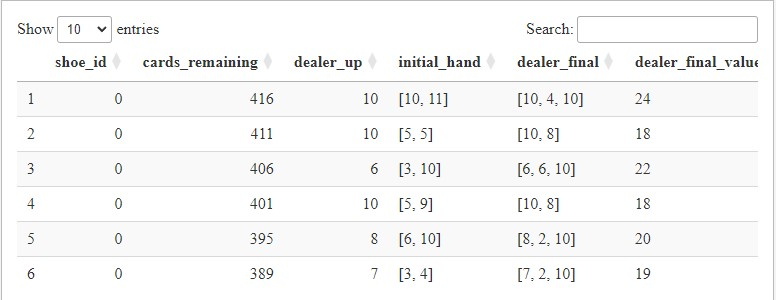
\includegraphics[width=2.5in]{C:/Users/USER/Documents/Proyecto minería/Capturas/Datos 1.jpg}
\DeclareGraphicsExtensions.
\caption{Primer vistazo del data sets con 50 millones de datos}
\label{Dataset}
\end{figure}

En la figura 1, se llevará a cabo una inspección preliminar que
permitirá identificar posibles valores atípicos o inconsistencias que
puedan requerir limpieza. Además, se generará una figura visual que
facilitará este análisis inicial, proporcionando un primer vistazo de
las características del conjunto de datos antes de proceder a las
transformaciones más detalladas.

\begin{figure}[htbp]
\centering
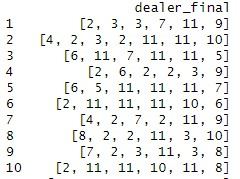
\includegraphics[width=2.5in]{C:/Users/USER/Documents/Proyecto minería/Capturas/Datos 2.jpg}
\DeclareGraphicsExtensions.
\caption{Columna con las cartas del dealer, la cual se usará en el procesamiento}
\label{Dataset 2}
\end{figure}

En la figura 2, se tomará una muestra representativa de 20,000 registros
del conjunto de datos original, utilizando una semilla (set.seed(123))
para garantizar la reproducibilidad de los resultados. A continuación,
se filtrarán aquellos registros donde la columna dealer\_final contenga
más de 4 valores separados por comas, lo que podría indicar manos
complejas o inusuales del crupier esto con el fin de entender el máximo
de cartas que podrían contener para ver la viabilidad de su división por
columnas independientes. A continuación, se dividirá la columna de
initial\_hand, la cual contiene las cartas iniciales del jugador y
posterior a ello se tratará la columna dealer\_final.

\begin{figure}[htbp]
\centering
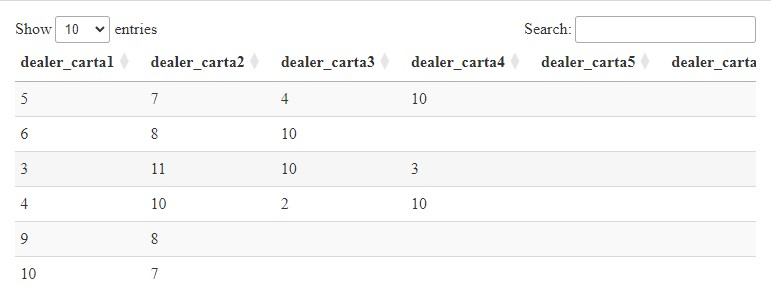
\includegraphics[width=2.5in]{C:/Users/USER/Documents/Proyecto minería/Capturas/Datos 3.jpg}
\DeclareGraphicsExtensions.
\caption{Dataset con la mano inicial del dealer en distintas columnas}
\label{Dataset 3}
\end{figure}

El la figura 3, se transformará la columna initial\_hand para eliminar
los corchetes que rodean los valores, asegurando que los datos estén en
un formato más limpio y manejable. Luego, se procederá a separar esta
columna en dos nuevas variables, carta1 y carta2, dividiendo los valores
por la coma que separa las cartas en la mano inicial. Este paso
permitirá analizar cada carta por separado, facilitando el análisis y
procesamiento de las manos iniciales en el juego. En el siguiente paso
se dividirá la mano final del dealer, con el fin, de tener una
perspectiva por columna, dado que el máximo de cartas que podrá tener el
dealer serán de 7 habrá filas donde se muestre un 0, el significado es
que el dealer no sacó más cartas.

\begin{figure}[htbp]
\centering
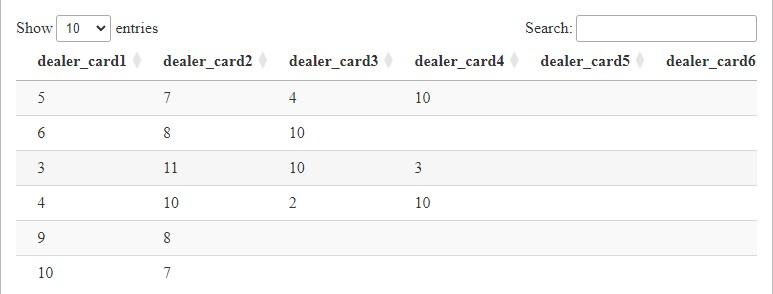
\includegraphics[width=2.5in]{C:/Users/USER/Documents/Proyecto minería/Capturas/Datos 4.jpg}
\DeclareGraphicsExtensions.
\caption{Dataset con las cartas del dealer por separado}
\label{Dataset 4}
\end{figure}

En la figura 4, se procederá a limpiar la columna dealer\_final,
eliminando los corchetes que rodean los valores para que los datos del
crupier estén en un formato adecuado para su análisis. Luego, se
separará esta columna en varias nuevas variables: dealer\_card1,
dealer\_card2, dealer\_card3, dealer\_card4, dealer\_card5,
dealer\_card6 y dealer\_card7, asignando cada carta a una columna
diferente. La separación se hará utilizando la coma como delimitador, y
se rellenarán las columnas que no tengan suficientes cartas con valores
vacíos. Este proceso permitirá analizar cada una de las cartas que el
crupier tiene en su mano final, proporcionando un mayor nivel de detalle
para el análisis posterior. Por último, se dejará más claro en español
las acciones que se tomaron en esa ronda.

\begin{figure}[htbp]
\centering
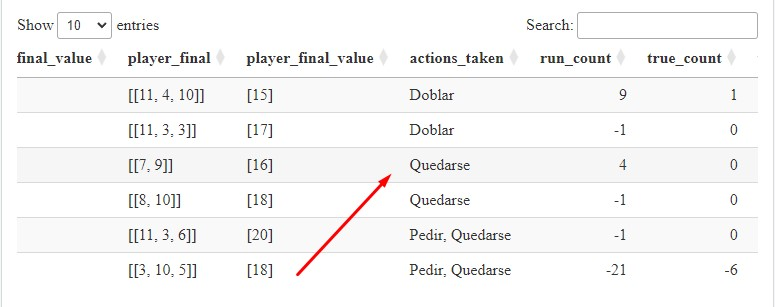
\includegraphics[width=2.5in]{C:/Users/USER/Documents/Proyecto minería/Capturas/Datos 5.jpg}
\DeclareGraphicsExtensions.
\caption{Dataset con las acciones por ronda más claras}
\label{Dataset 5}
\end{figure}

En la figura 5, se define una función llamada
replace\_actions\_multiple, cuyo objetivo es transformar los códigos de
acciones registrados en la columna actions\_taken en descripciones más
comprensibles. Esta función divide cada conjunto de acciones por comas y
luego reemplaza cada código con su correspondiente acción en español,
utilizando la función case\_when. Las acciones codificadas, como ``H''
(Pedir), ``S'' (Quedarse), ``D'' (Doblar), entre otras, se convierten en
sus descripciones completas Hewig et al. (2007). Posteriormente, la
función reconstruye la lista de acciones reemplazadas en un solo texto,
manteniendo el formato original.

Finalmente, se aplica esta función a la columna actions\_taken del
conjunto de datos, limpiando primero los corchetes y apóstrofes que
rodean los valores. Este proceso facilita la interpretación de las
acciones tomadas durante el juego, permitiendo que se trabaje con datos
más claros y legibles en los siguientes análisis.

\begin{figure}[htbp]
\centering
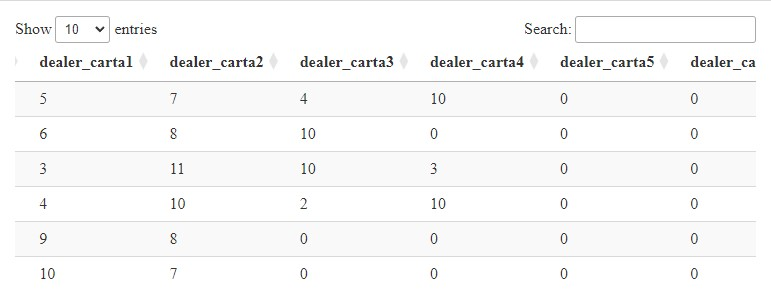
\includegraphics[width=2.5in]{C:/Users/USER/Documents/Proyecto minería/Capturas/Datos 6.jpg}
\DeclareGraphicsExtensions.
\caption{Dataset con los 0 correspondientes, lo cual señala, la ausencia de una carta}
\label{Dataset 6}
\end{figure}

En la figura 6, se procede a manejar los valores faltantes dentro del
conjunto de datos. Para las columnas numéricas, se reemplazan los
valores NA con ceros, lo que asegura que los cálculos y análisis futuros
no se vean afectados por valores vacíos en dichas columnas. De manera
similar, en las columnas de tipo carácter, los valores NA se sustituyen
por ``0'', lo que estandariza el tratamiento de los datos faltantes y
evita problemas en procesos posteriores de manipulación o visualización.
Esta estrategia garantiza que no queden valores faltantes que puedan
generar errores o interpretaciones incorrectas en el análisis.

\begin{figure}[htbp]
\centering
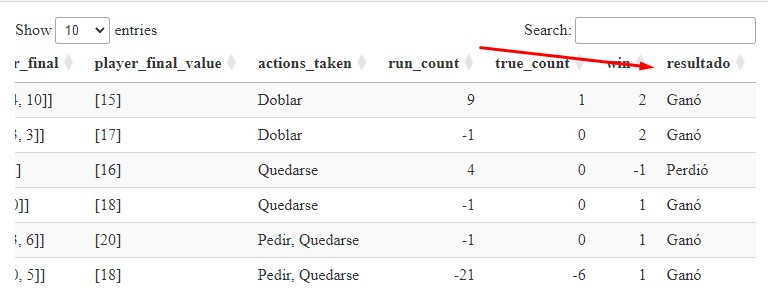
\includegraphics[width=2.5in]{C:/Users/USER/Documents/Proyecto minería/Capturas/Datos 7.jpg}
\DeclareGraphicsExtensions.
\caption{Dataset con la nueva columna de resultados}
\label{Dataset 7}
\end{figure}

En la figura 7, se crea una nueva columna llamada resultado que
clasifica el resultado de cada jugada según los valores de la columna
win. Se utiliza la función case\_when para asignar etiquetas
descriptivas basadas en el valor de la variable win: si el valor es
negativo (win \textless{} 0), el jugador ``Perdió''; si es cero (win ==
0), el jugador ``Empató''; y si es positivo (win \textgreater{} 0), el
jugador ``Ganó''. Esta nueva columna facilita la interpretación de los
resultados del juego, permitiendo un análisis más claro y directo de las
jugadas.

\section{Minería de datos}\label{mineruxeda-de-datos}

La minería de datos es el proceso de descubrir patrones, correlaciones y
tendencias dentro de grandes volúmenes de datos, utilizando técnicas de
análisis avanzado. En este proyecto, aplicaremos minería de datos a un
conjunto de datos de Blackjack para entender cómo diferentes factores
(como las cartas en mano del jugador y del dealer, así como las acciones
tomadas) afectan el resultado de la partida. El objetivo final es
construir un modelo que pueda predecir estos resultados y así ayudar a
tomar decisiones estratégicas.

Utilizaremos redes neuronales para crear un modelo que pueda aprender
patrones en los datos y realizar predicciones. Las redes neuronales son
modelos de aprendizaje profundo que se inspiran en el funcionamiento del
cerebro humano, donde múltiples ``neuronas'' (unidades de procesamiento)
están conectadas y trabajan en conjunto para procesar datos y encontrar
patrones. Son especialmente útiles en problemas complejos como este, ya
que permiten capturar relaciones no lineales entre las variables.

El primer paso es asegurarnos de que la variable resultado, que
representa el resultado final del juego (ganar, perder, empatar), se
trata como un factor en lugar de un valor numérico, además, analizará
4000 datos para evitar que la red neuronal tarde demasiado en el
procesamiento. Esto es importante porque queremos que el modelo prediga
categorías (clasificación) y no valores continuos. Luego seleccionaremos
solo las columnas relevantes para el modelo, excluyendo datos
adicionales que no aporten información para el entrenamiento de la red
neuronal. Esto incluye las cartas del jugador y el dealer, el valor
final del dealer, las acciones tomadas por el jugador y el resultado
final.

\begin{figure}[htbp]
\centering
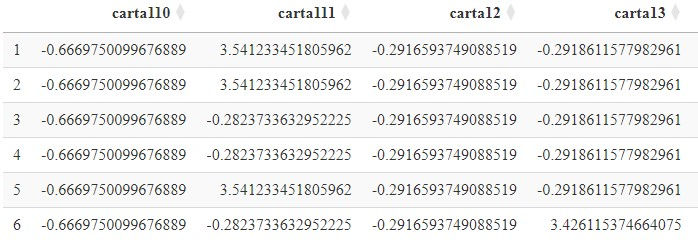
\includegraphics[width=2.5in]{C:/Users/USER/Documents/Proyecto minería/Capturas/Mineria 1.jpg}
\DeclareGraphicsExtensions.
\caption{Dataset con variables dummy para las columnas a trabajar}
\label{Mineria 1}
\end{figure}

En la figura 8, se observan las variables dummy que permiten transformar
las variables categóricas en un formato numérico, que es más adecuado
para el modelo. Por ejemplo, si actions\_taken tiene valores como
``hit'' y ``stand'', el modelo las convierte en variables
numéricas.Además, se escalan los datos significa normalizar todas las
variables para que tengan una media de 0 y una desviación estándar de 1.
Esto es crucial para el entrenamiento de la red neuronal, ya que evita
que variables con valores grandes dominen el aprendizaje del modelo y
permite que el entrenamiento sea más estable y rápido. Esto es crucial
para el entrenamiento de la red neuronal, ya que evita que variables con
valores grandes dominen el aprendizaje del modelo y permite que el
entrenamiento sea más estable y rápido.Finalmente, se divide el conjunto
de datos en dos partes: entrenamiento (80\%) y prueba (20\%). El modelo
se entrena en los datos de entrenamiento y se evalúa en los datos de
prueba para medir su capacidad de generalización.

\begin{figure}[htbp]
\centering
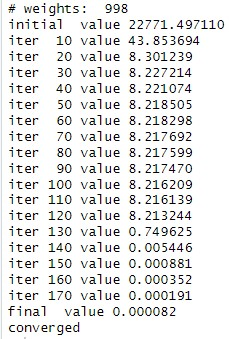
\includegraphics[width=2.5in]{C:/Users/USER/Documents/Proyecto minería/Capturas/Mineria 2.jpg}
\DeclareGraphicsExtensions.
\caption{Proceso de entrenamiento de la red neuronal}
\label{Mineria 2}
\end{figure}

En la figura 9, después de definir el modelo, comienza el proceso de
entrenamiento u optimización de la red neuronal, donde se ajustan los
pesos de las conexiones entre neuronas en cada iteración para minimizar
el error entre las predicciones del modelo y los valores reales en
train\_data. Con un total de 998 pesos ajustables (que representan las
conexiones entre las neuronas de las diferentes capas), el proceso
inicia con un valor de pérdida inicial alto, que luego disminuye a
medida que la red ajusta sus pesos en cada iteración. Por ejemplo, en la
iteración 10, el valor de la función de pérdida es de 43.85, y continúa
descendiendo hasta llegar a 0.000082 al final del entrenamiento. Este
valor final, bastante bajo, sugiere que el modelo ha aprendido bien los
patrones en los datos de entrenamiento. El mensaje ``converged'' indica
que la optimización ha alcanzado un punto donde el modelo ya no mejora
significativamente con más iteraciones, por lo que el proceso se detiene
antes de alcanzar el límite de maxit = 200. En resumen, el entrenamiento
de la red busca minimizar el error de predicción usando los datos de
entrenamiento, y el modelo resultante está listo para evaluarse en datos
no vistos, como test\_data.

\begin{figure}[htbp]
\centering
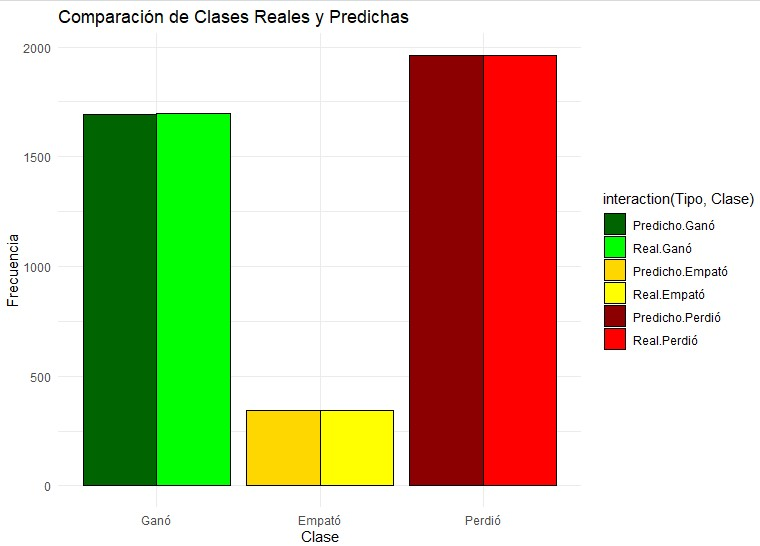
\includegraphics[width=2.5in]{C:/Users/USER/Documents/Proyecto minería/Capturas/Mineria 3.jpg}
\DeclareGraphicsExtensions.
\caption{Comparación de resultados entre el resultado real y la predicha por la red neuronal}
\label{Mineria 3}
\end{figure}

En la figura 10, se puede observar una comparación entre los resultados
reales y la predicción que realizó la red neuronal. El resultado se hizo
a través de un vector llamado predicciones que contiene las clases
predichas por el modelo para cada fila de test\_data. Estas predicciones
representan el resultado que la red neuronal cree que ocurrirá en cada
partida de Blackjack según las características que ya conoce. Luego,
estas predicciones se pueden comparar con los resultados reales para
evaluar la precisión y el rendimiento del modelo. Al observar el gráfico
se puede observar que hay unos pequeños datos que no coinciden con
valores reales.

\begin{figure}[htbp]
\centering
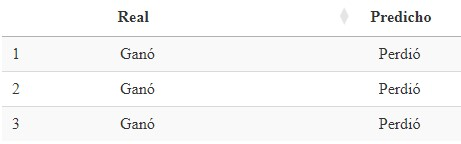
\includegraphics[width=2.5in]{C:/Users/USER/Documents/Proyecto minería/Capturas/Mineria 4.jpg}
\DeclareGraphicsExtensions.
\caption{Datos que no coinciden}
\label{Mineria 4}
\end{figure}

En la figura 11, se observan y filtran los datos donde se generaron
cambios. Esto pequeño cambio se debe a partidas demasiado únicas con un
contexto de decisiones muy amplio, donde la red, no tiene la suficiente
información para manejar división de manos con diferentes opciones, dado
que la cantidad es tan mínima se considera que no tiene relevancia dado
que el modelo pudo predecir los demás juegos sin problema alguna a pesar
de también tener una gran cantidad de decisiones de por medio.

\begin{figure}[htbp]
\centering
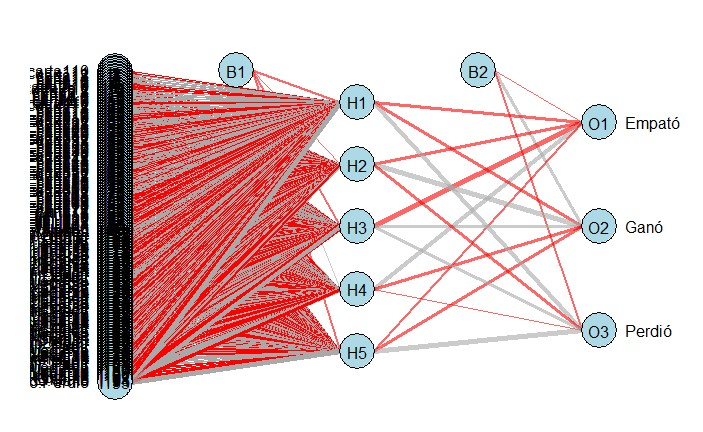
\includegraphics[width=2.5in]{C:/Users/USER/Documents/Proyecto minería/Capturas/Red neuronal.jpg}
\DeclareGraphicsExtensions.
\caption{Imagen de la red neuronal}
\label{Red neuronal}
\end{figure}

En la figura 12 se observa la capa de entrada, ubicada a la izquierda
del gráfico, contiene una gran cantidad de variables. Estas entradas
representan las características o variables del modelo de red neuronal,
que probablemente están relacionadas con las jugadas y decisiones en el
contexto del Blackjack. Las conexiones rojas que parten de esta capa
indican cómo cada una de estas variables de entrada se conecta con las
neuronas de la siguiente capa, que es la capa oculta.

En el centro, encontramos la capa oculta, compuesta por cinco neuronas,
etiquetadas como H1, H2, H3, H4 y H5. Estas neuronas realizan
combinaciones lineales de las entradas ponderadas y aplican una función
de activación para generar su salida. Las conexiones de colores reflejan
el signo de los pesos: las conexiones en rojo representan pesos
negativos, mientras que las conexiones en gris indican pesos positivos.
Además, el grosor y la intensidad de las líneas reflejan la magnitud de
los pesos: conexiones más gruesas e intensas indican un peso mayor en
valor absoluto, lo que implica que tienen un impacto significativo en la
activación de la neurona destino.

La capa de salida, a la derecha del gráfico, consta de tres neuronas
etiquetadas como O1 (Empató), O2 (Ganó) y O3 (Perdió). Cada una de estas
neuronas representa una posible clase para la predicción final del
modelo. En este caso, el objetivo de la red es clasificar el resultado
de una partida de Blackjack en una de estas tres categorías, lo que
sugiere un problema de clasificación multinomial en el que el modelo
decide entre tres posibles resultados basándose en las activaciones de
la capa oculta.

Las neuronas B1 y B2 representan los términos de sesgo (bias) en la capa
oculta y en la capa de salida, respectivamente. Estas neuronas de sesgo
son constantes y están conectadas a todas las neuronas de sus
respectivas capas. Los términos de sesgo permiten que la red ajuste el
punto de activación de las neuronas, ayudando a que el modelo se ajuste
mejor a los datos al desplazar la función de activación de cada neurona
y, por ende, mejorar la precisión de las predicciones.

\section{Evaluación de los datos}\label{evaluaciuxf3n-de-los-datos}

\begin{figure}[htbp]
\centering
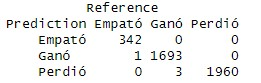
\includegraphics[width=2.5in]{C:/Users/USER/Documents/Proyecto minería/Capturas/Mineria 5.jpg}
\DeclareGraphicsExtensions.
\caption{Estadísiticas de la matriz de confusión}
\label{Mineria 5}
\end{figure}

El modelo tiene un rendimiento sobresaliente, como lo indica la matriz
de confusión, también conocida como matriz de error, es un instrumento
tecnológico que sirve para calcular el rendimiento sobre un modelo de
clasificación definido DataScientest (2024) como se observa en la figura
13, que muestra cómo las predicciones se distribuyen entre las clases
reales (``Empató'', ``Ganó'' y ``Perdió'') en comparación con las
predicciones realizadas por el modelo. En la clase Empató, el modelo
clasificó correctamente 342 casos como ``Empató'' y no cometió errores,
ya que no predijo incorrectamente como ``Ganó'' ni ``Perdió''. Esto
refleja una alta precisión para esta clase. En la clase Ganó, el modelo
predijo correctamente 1693 casos como ``Ganó'', aunque cometió un
pequeño error al predecir un caso como ``Ganó'' cuando realmente fue
``Empató''. Finalmente, en la clase Perdió, el modelo también tuvo un
excelente desempeño, con 1960 casos correctamente clasificados y solo
tres errores de predicción en los que predijo ``Ganó'' en lugar de
``Perdió''.

\begin{figure}[htbp]
\centering
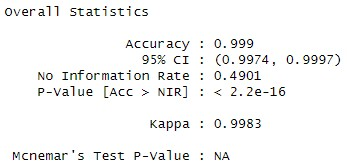
\includegraphics[width=2.5in]{C:/Users/USER/Documents/Proyecto minería/Capturas/Mineria 6.jpg}
\DeclareGraphicsExtensions.
\caption{Estadísiticas extra de la matriz de confusión}
\label{Mineria 6}
\end{figure}

En la figura 14, el índice de exactitud es de 0.999 (99.9\%), lo que
sugiere que el modelo acertó en casi todas las predicciones realizadas.
Además, el intervalo de confianza del 95\% para la exactitud varía entre
99.74\% y 99.97\%, lo que indica que la estimación de la exactitud es
robusta y confiable. Este alto valor de exactitud es aún más
significativo dado que la tasa de no información (No Information Rate)
es de 0.4901, lo que representa la proporción de la clase mayoritaria en
los datos. El modelo supera ampliamente esta tasa, lo que demuestra que
no solo está prediciendo correctamente la clase mayoritaria, sino que
también tiene una alta capacidad para clasificar correctamente las
clases minoritarias.

En términos de la estadística de Kappa, que mide la concordancia entre
las predicciones del modelo y las clases reales, el valor de 0.9983
indica una excelente concordancia, mucho mejor que lo que se esperaría
por azar. Esto confirma que el modelo no solo está funcionando bien en
términos de precisión general, sino que las predicciones son
consistentes con las clases reales.

\begin{figure}[htbp]
\centering
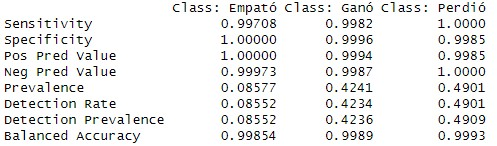
\includegraphics[width=2.5in]{C:/Users/USER/Documents/Proyecto minería/Capturas/Mineria 7.jpg}
\DeclareGraphicsExtensions.
\caption{Estadísiticas por clase de la matriz de confusión}
\label{Mineria 7}
\end{figure}

En la figura 15, las métricas por clase proporcionan un análisis
detallado del rendimiento del modelo en cada una de las clases. Para la
clase Empató, la sensibilidad es del 99.7\%, lo que significa que el
modelo detectó correctamente el 99.7\% de los casos que realmente fueron
``Empató''. Además, la especificidad es del 100\%, lo que indica que no
hubo falsos positivos para esta clase. El valor predictivo positivo
también es perfecto, con un 100\%, lo que significa que cuando el modelo
predijo ``Empató'', estaba correcto en todas las ocasiones. La
prevalencia de esta clase es relativamente baja, con solo un 8.58\% de
los casos pertenecientes a ``Empató'', lo que hace aún más impresionante
el alto desempeño del modelo en esta clase minoritaria.

En cuanto a la clase Ganó, la sensibilidad es de 99.8\%, lo que indica
que el modelo identificó correctamente el 99.8\% de los casos ganadores.
La especificidad es de 99.96\%, lo que significa que el modelo detectó
correctamente los casos que no eran ``Ganó'' en casi todos los casos.
Los valores predictivos positivos y negativos también son muy altos, con
un 99.94\% y un 99.87\%, respectivamente. La prevalencia de esta clase
es del 42.41\%, lo que la convierte en la clase mayoritaria en los
datos.

Por último, en la clase Perdió, el modelo tuvo un desempeño perfecto en
términos de sensibilidad y especificidad, con 100\% en ambas métricas.
Esto significa que el modelo identificó correctamente todos los casos
perdedores y no cometió errores al clasificar las otras clases como
``Perdió''. El valor predictivo positivo es del 99.85\% y el valor
predictivo negativo es del 100\%, lo que refleja un rendimiento muy
sólido. La prevalencia de esta clase es del 49.01\%, lo que la convierte
en la clase más frecuente en el conjunto de datos.

\begin{figure}[htbp]
\centering
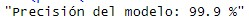
\includegraphics[width=2.5in]{C:/Users/USER/Documents/Proyecto minería/Capturas/Mineria 8.jpg}
\DeclareGraphicsExtensions.
\caption{Porcentaje de precisión}
\label{Mineria 8}
\end{figure}

El modelo tiene una precisión del 99.9\% según la figura 16, lo que
indica que las predicciones realizadas por el modelo son correctas en un
porcentaje muy alto de las veces. Este valor sugiere que el modelo está
funcionando muy bien, especialmente en tareas con un alto número de
datos de prueba. Sin embargo, es importante también considerar otras
métricas, como la sensibilidad, especificidad, o el valor predictivo
positivo, para tener una visión más completa del rendimiento del modelo
como se explicó en las anteriores figuras.

¿Cuáles son las decisiones más efectivas basadas en la mano del jugador
y la carta visible del dealer? ¿Cómo varían las probabilidades de ganar
dependiendo de las decisiones tomadas en diferentes situaciones? y
¿Existen patrones repetitivos en las manos repartidas que se puedan
aprovechar para mejorar la estrategia del jugador?

Para responder estás preguntas, se usarán los siguientes gráficos y
estadísticas.

\begin{figure}[htbp]
\centering
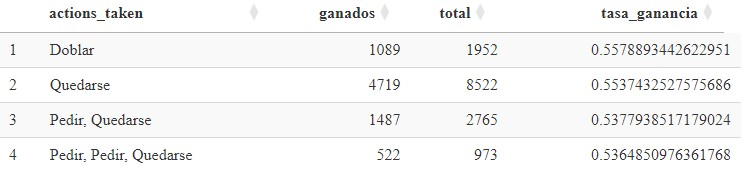
\includegraphics[width=2.5in]{C:/Users/USER/Documents/Proyecto minería/Capturas/Mineria 9.jpg}
\DeclareGraphicsExtensions.
\caption{Acciones más utilizadas junto con su tasa de ganancia y total de juegos}
\label{Mineria 9}
\end{figure}

Según la figura 17, podemos ver:

\begin{enumerate}
\def\labelenumi{\arabic{enumi}.}
\item
  Acción más exitosa: ``Doblar'' Ganados: 1,089 Total: 1,952 Tasa de
  Ganancia: 55.8\% La acción ``Doblar'' es la que tiene la tasa de
  ganancia más alta, con un 55.8\%. Esto indica que, en promedio, cuando
  un jugador decide doblar su apuesta, tiene más probabilidades de
  ganar. Aunque no es la acción más frecuente (tiene menos total de
  partidas que ``Quedarse''), tiene un buen rendimiento en términos de
  éxito relativo.
\item
  Acción más frecuente: ``Quedarse'' Ganados: 4,719 Total: 8,522 Tasa de
  Ganancia: 55.4\% La acción ``Quedarse'' es la más común, con más de
  8,500 partidas registradas. Su tasa de ganancia es muy similar a la de
  ``Doblar'' (55.4\%), lo que sugiere que, en términos de cantidad de
  partidas, esta es una acción que también tiene un rendimiento bastante
  bueno. Aunque no tiene la tasa de ganancia más alta, al ser tan
  frecuente, es una estrategia sólida para los jugadores.
\item
  Acción combinada: ``Pedir, Quedarse'' Ganados: 1,487 Total: 2,765 Tasa
  de Ganancia: 53.8\% Esta acción combina ``Pedir'' y luego
  ``Quedarse''. Tiene una tasa de ganancia de 53.8\%, ligeramente
  inferior a las anteriores, pero sigue siendo una estrategia bastante
  efectiva en términos de éxito. Sin embargo, tiene un total de partidas
  más bajo en comparación con las dos primeras acciones, lo que podría
  reflejar un estilo de juego menos frecuente o específico.
\item
  Acción más riesgosa: ``Pedir, Pedir, Quedarse'' Ganados: 522 Total:
  973 Tasa de Ganancia: 53.6\% La acción de pedir dos veces antes de
  quedarse (``Pedir, Pedir, Quedarse'') tiene una tasa de ganancia de
  53.6\%, que es la más baja entre las acciones analizadas, pero sigue
  siendo relativamente alta. Sin embargo, el número de partidas es
  también menor, lo que puede indicar que esta es una estrategia menos
  adoptada por los jugadores, o que se utiliza solo en situaciones
  específicas.
\end{enumerate}

Claramente, cada sección está sujeta a las cartas que se tengan en
juego, al ser un juego donde no conoces aún las cartas que tendras.En
ese caso, se mostrarán las dos primeras acciones la combinación de
cartas que fue más efectiva.

\begin{figure}[htbp]
\centering
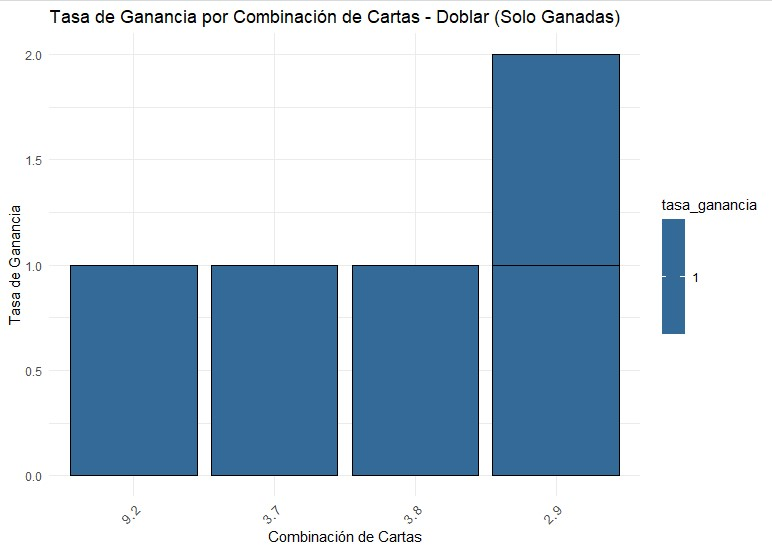
\includegraphics[width=2.5in]{C:/Users/USER/Documents/Proyecto minería/Capturas/Eva 1.jpg}
\DeclareGraphicsExtensions.
\caption{Cartas más frecuentes en Doblar}
\label{Evaluacion 1}
\end{figure}

Dada la figura 18, se observa que al doblar lo más común es tomar el
riesgo cuando se tiene un 9 y un 2, siendo la tasa más alta de victoria.

\begin{figure}[htbp]
\centering
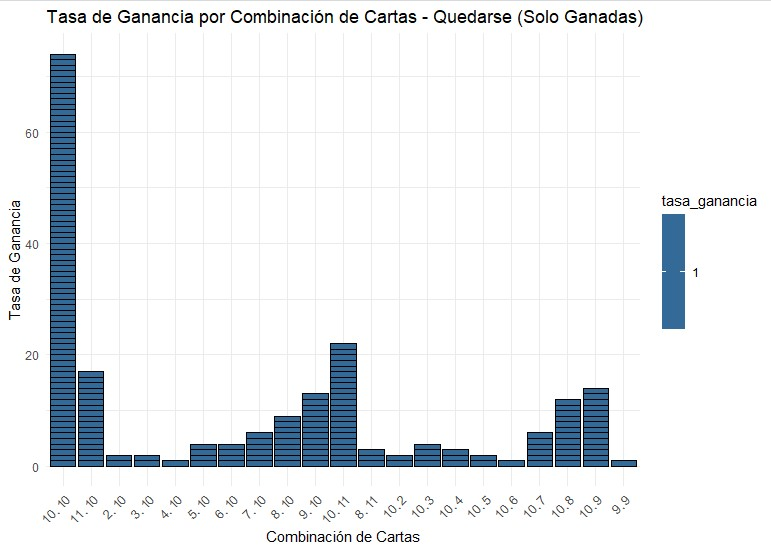
\includegraphics[width=2.5in]{C:/Users/USER/Documents/Proyecto minería/Capturas/Eva 2.jpg}
\DeclareGraphicsExtensions.
\caption{Cartas más frecuentes en Quedarse}
\label{Evaluacion 2}
\end{figure}

Según la figura 19, se observa que las combinaciones entre (10, 10),
(9,10) y en general, combinaciones con el número 10 y un número mayor a
7 tiene una tasa de victoria más alta al quedarse.

\newpage

\section{Anexos}\label{anexos}

Las figuras mostradas a continuación tienen como fin mostrar que el
proceso de transformación permite la manipulación de los datos de una
manera más optima para el proyecto, permitiendo dar ejemplos de
gráficos.

\begin{figure}[htbp]
\centering
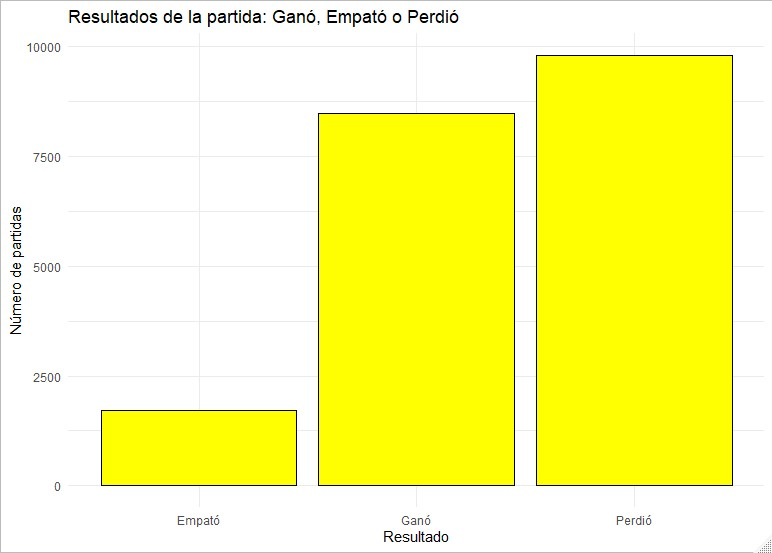
\includegraphics[width=2.5in]{C:/Users/USER/Documents/Proyecto minería/Capturas/Grafica 1.jpg}
\DeclareGraphicsExtensions.
\caption{Gráfica de barras a raíz de la nueva columna resultado}
\label{Dataset 8}
\end{figure}

En la figura 20, Se crea un gráfico de barras donde el eje x muestra las
categorías de resultado (``Ganó'', ``Empató'' y ``Perdió'') y el eje y
indica el número de partidas en cada categoría. Las barras se colorean
de amarillo con bordes negros para destacar los resultados. Además, se
añaden etiquetas al gráfico, incluyendo un título que describe la
visualización y etiquetas para los ejes, lo que facilita la comprensión
de la información presentada. Este gráfico proporciona una visión
general del desempeño del jugador en las partidas, permitiendo
identificar patrones y tendencias en los resultados. Se observa que el
resultado más común es perder, sin embargo, no está muy lejos del
resultado de ganar.

\begin{figure}[htbp]
\centering
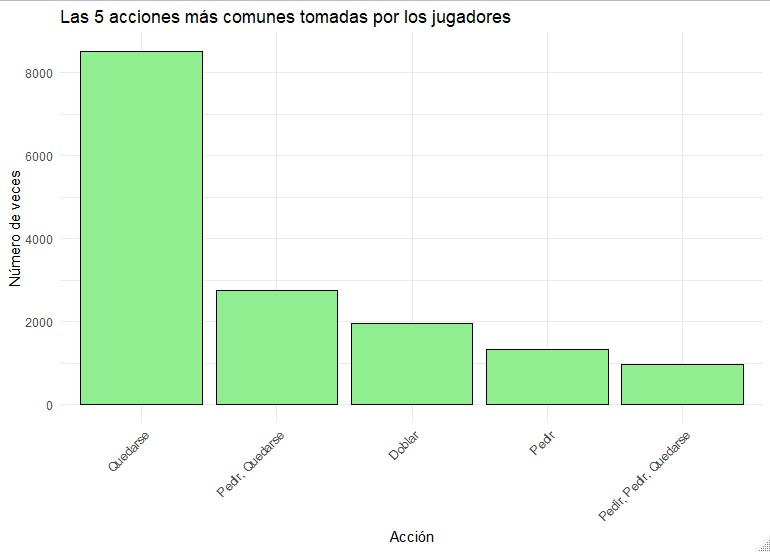
\includegraphics[width=2.5in]{C:/Users/USER/Documents/Proyecto minería/Capturas/Grafico 2.jpg}
\DeclareGraphicsExtensions.
\caption{Gráfica con las acciones más frecuentes por los jugadores}
\label{Dataset 9}
\end{figure}

En la figura 21, se identifican las acciones más frecuentes tomadas por
los jugadores durante las partidas. Para ello, se agrupan los datos por
la columna actions\_taken, se cuenta el número de ocurrencias de cada
acción utilizando summarise, y se ordenan los resultados de forma
descendente. Posteriormente, se seleccionan las cinco acciones más
comunes mediante la función slice\_max.

En el gráfico de barras, el eje x muestra las acciones reordenadas según
su frecuencia, mientras que el eje y indica el número de veces que cada
acción fue tomada. Las barras se colorean de verde claro con bordes
negros para hacer la visualización más atractiva. Se añaden etiquetas al
gráfico, incluyendo un título y descripciones para los ejes, y se ajusta
la orientación del texto en el eje x para mejorar la legibilidad. Esta
visualización permite analizar de manera clara las acciones más comunes
que los jugadores realizan, proporcionando información valiosa sobre su
comportamiento durante el juego. Se puede observar con gran diferencia
que los jugadores deciden quedarse más frecuentemente, lo que indica, no
tomar riesgos.

\begin{figure}[htbp]
\centering
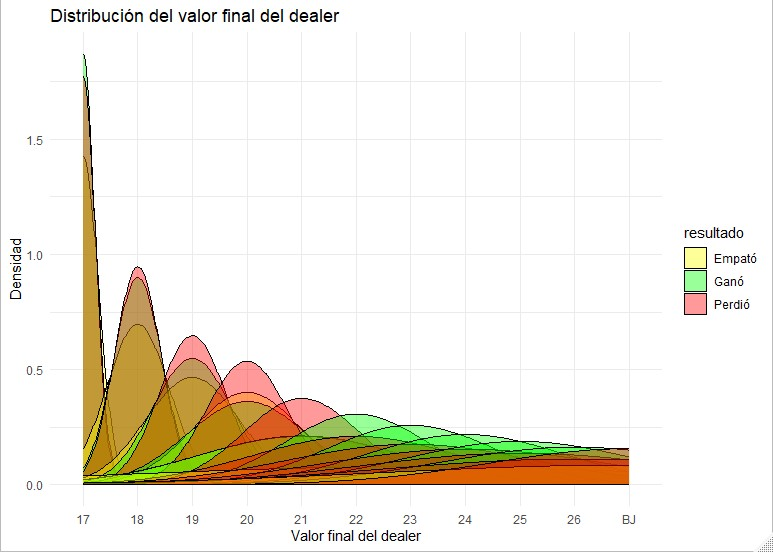
\includegraphics[width=2.5in]{C:/Users/USER/Documents/Proyecto minería/Capturas/Grafica 3.jpg}
\DeclareGraphicsExtensions.
\caption{Gráfica de calor respecto al resultado del jugador}
\label{Dataset 10}
\end{figure}

En la figura 22, se elabora una visualización de la distribución del
valor final del crupier utilizando un gráfico de densidad. En este
gráfico, el eje x representa el valor final del crupier
(dealer\_final\_value), mientras que el eje y indica la densidad de los
valores observados. Las áreas bajo la curva se llenan con diferentes
colores según el resultado de la partida, permitiendo distinguir
fácilmente entre las categorías ``Ganó'', ``Empató'' y ``Perdió''.

La opacidad de las áreas se ajusta con un valor alfa de 0.4, lo que
permite una mejor visualización de las superposiciones. Se añaden
etiquetas descriptivas, incluyendo un título que refleja el contenido
del gráfico y etiquetas para los ejes, para una mejor comprensión.
Además, se utiliza scale\_fill\_manual para asignar colores específicos
a cada resultado: verde para ``Ganó'', amarillo para ``Empató'' y rojo
para ``Perdió''. Esta visualización proporciona una visión clara de cómo
se distribuyen los valores finales del crupier en relación con los
resultados de las partidas, facilitando la identificación de tendencias
y patrones en los datos.

\begin{figure}[htbp]
\centering
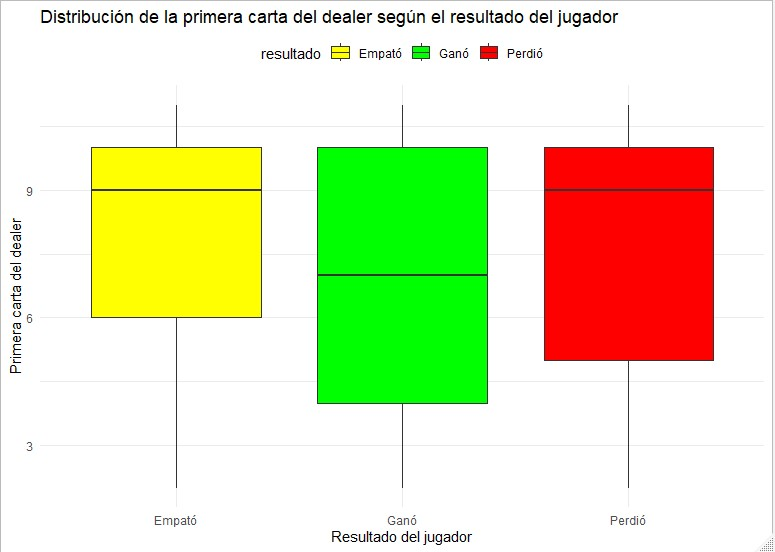
\includegraphics[width=2.5in]{C:/Users/USER/Documents/Proyecto minería/Capturas/Grafico 4.jpg}
\DeclareGraphicsExtensions.
\caption{Boxplot que visualiza según la carta, donde se encuentran reunidos más los datos donde ganó, perdió o empató}
\label{Dataset 11}
\end{figure}

En la figura 23, se crea un gráfico de cajas (boxplot) para analizar la
distribución de la primera carta del crupier (dealer\_carta1) en función
del resultado del jugador. En el gráfico, el eje x representa los
resultados (``Ganó'', ``Empató'' y ``Perdió''), mientras que el eje y
muestra los valores de la primera carta del crupier.

Se utilizan colores específicos para rellenar las cajas según el
resultado del jugador, y los valores atípicos se resaltan en rojo para
facilitar su identificación. Además, se añaden etiquetas que incluyen un
título descriptivo y nombres para los ejes, lo que mejora la comprensión
del gráfico. La función scale\_fill\_manual se emplea para asignar
colores particulares: verde para ``Ganó'', amarillo para ``Empató'' y
rojo para ``Perdió''. Por último, se posiciona la leyenda en la parte
superior del gráfico para que sea fácilmente visible. Esta visualización
permite observar cómo varía la primera carta del crupier en relación con
el desempeño del jugador, facilitando la identificación de patrones y
posibles correlaciones entre las cartas y los resultados del juego.

\section{Conclusiones}\label{conclusiones}

El análisis realizado demuestra que el uso de minería de datos y redes
neuronales es eficaz para modelar y evaluar decisiones estratégicas en
Blackjack. A través del proceso de KDD, fue posible transformar un
conjunto de datos brutos en un modelo de red neuronal capaz de
identificar patrones y decisiones óptimas en el juego. El enfoque
utilizado en este proyecto ha permitido no solo predecir resultados en
función de las decisiones del jugador, sino también entender los
factores que influyen en dichas decisiones, proporcionando una visión
más profunda sobre la dinámica del juego.

La visualización de las activaciones y los pesos en las capas de la red
neuronal resultó ser una herramienta valiosa para evaluar la lógica del
modelo y analizar cómo responde ante diferentes configuraciones de
cartas y jugadas. Este análisis detallado de la red neuronal revela
patrones específicos que corresponden a decisiones estratégicas, como
cuándo es más probable que un jugador gane, pierda o empate. Asimismo,
el uso de variables dummy y la normalización de los datos aseguraron que
el modelo tuviera una representación clara y consistente de cada estado
del juego, optimizando su capacidad de generalizar las decisiones en
diferentes escenarios.

Además, el proyecto resalta la versatilidad de los modelos de redes
neuronales en problemas de toma de decisiones complejas en entornos
inciertos. La metodología presentada puede ser aplicada a otros juegos o
contextos donde la estrategia y la probabilidad juegan un rol
importante, como en la gestión de riesgos financieros o la toma de
decisiones en entornos empresariales. En última instancia, este proyecto
demuestra que la combinación de minería de datos y aprendizaje puede
ofrecer soluciones innovadoras y efectivas en la optimización de
decisiones estratégicas en Blackjack e incluso otros juegos.

Estos resultados permiten la optimización del modelo a través de la
inclusión de más capas o neuronas, o la experimentación con técnicas de
regularización para mejorar su rendimiento. En conclusión, este proyecto
no solo contribuye a la comprensión de estrategias en Blackjack, sino
que también destaca el potencial de las redes neuronales y la minería de
datos para resolver problemas complejos de manera efectiva, demostrando
el poder del aprendizaje automático en el análisis de decisiones
estratégicas.

\newpage

\section*{References}\label{references}
\addcontentsline{toc}{section}{References}

\phantomsection\label{refs}
\begin{CSLReferences}{1}{0}
\bibitem[\citeproctext]{ref-Cotte2009742}
Cotte, June, and Kathryn A. Latour. 2009. {``Blackjack in the Kitchen:
Understanding Online Versus Casino Gambling.''} \emph{The Journal of
Consumer Research} 35 (5): 742--58.

\bibitem[\citeproctext]{ref-DataScientest2024}
DataScientest. 2024. {``Matriz de Confusión.''} 2024.
\url{https://datascientest.com/es/matriz-de-confusion}.

\bibitem[\citeproctext]{ref-Hewig2007865}
Hewig, Johannes, Ralf Trippe, Holger Hecht, Michael G. H. Coles, Clay B.
Holroyd, and Wolfgang H. R. Miltner. 2007. {``Decision-Making in
Blackjack: An Electrophysiological Analysis.''} \emph{Cerebral Cortex}
17 (4): 865--77.

\bibitem[\citeproctext]{ref-Venetian2024}
Resort, The Venetian. n.d. {``Blackjack Basics.''}
\url{https://www.venetianlasvegas.com/resort/casino/table-games/how-to-play-blackjack.html}.

\end{CSLReferences}

\end{document}

